\newcommand{\anfu}[1]{\glqq #1\grqq}
\newcommand{\anfuc}[3]{\anfu{#1}\cite[{#2}]{#3}}

\section{Architecture}
\subsection{Core Processes}\label{mdb-core}
The MongoDB server package comes up with three main processes:
\begin{itemize}
  \item mongod
  \item mongo
  \item mongos
\end{itemize}
\textit{Mongod} is the core database server. Once started, the \textit{mongod} listens by default on port 27017 for requests. It also manages the data format and performs all background operations. For administration the \textit{mondod} provides an HTTP interface, witch can be reached at the localhost on port 28017 (1000 higher than the default port). The data directory \textit{mongod} connects to is by default C:\textbackslash data\textbackslash db (or /data/db). This directory definitely has to exist and the default ports have to be free, otherwise the process fails to start \cite{Edward2015}.\\
The \textit{mongo} process is an interactive MongoDB shell. It gives the user the possibility to communicate with a running \textit{mongod} process via a JavaScript like query language. If running on the same host, it automatically connects to the \textit{mongod} process and a preinstalled test database \cite{Edward2015}.\\
The \textit{mongos} process is working like a routing service and is the basis for MongoDBs sharding ability that will be described later (\ref{mdb-sharding}). It holds the information about where the requested data is located and forwards the request from an application server to the right destination \cite{Edward2015}. \\
By running a \textit{mongod} process you already have a standalone deployment of MonogDB that can be accessed by a client. But in case of failure there is no redundancy or recovery, that prevents data loss, so its not recommended to use this in a production environment. To avoid this, replication is used to guard against hardware failure or database corruption. It also gives the possibility to perform normally high-impact maintenance with little or no impact \cite{Hows2013}.

\subsection{Replication}
\anfuc{MongoDB supports the replication of a database’s contents to another server in real time or near real time}{p. 285}{Hows2013}. For that MongoDB provides two different replication methods. The traditional \textit{Master/Slave Replication} and \textit{Replication Sets}.

\subsubsection{Master/Slave Replication}
In a Master/Slave setup one \textit{mongod} instance acts as a master, the others declared as slaves. All write and read operations are requested to the master and the slaves replicate the data of the master, but can't be requested by a client. If a failure occurs that forces the master to go down, the hole system can't be reached anymore. The data, till the last replication to the slaves, is saved, but can't be accessed until the master comes up again. \\
In MongoDB the master holds a capped collection called \textit{oplog}. The \textit{oplog} is an ordered history of all logical writes, that are executed within a defined time period. The operations stored in the \textit{oplog} in an idempotent way, so they can be performed multiple times without changing the result \cite{Edward2015}. That's useful when a slave runs into failure while executing the operations onto its data. In that case the replication process can be simply restarted. If the slaves syncing process last to long or the slave was down for a longer time, the oplog data could be deleted before the slave was able to synchronize \cite{Edward2015}. In that case the slave has to start a resync process. To avoid such a situation, the oplog length should be chosen in consideration of the slaves performance.\\
The configuration of MongoDB with a \textit{Master/Slave Replication} is only recommended for more than 50 nodes \cite{Edward2015}. At that point the next described replication method, the \textit{Replica Set}, is reaching its limits, because the communication overhead becomes to big.

\subsubsection{Replica sets}
In contrast to the \textit{Master/Slave Replication}, in a \textit{Replica Set} no fixed master is defined. Instead the nodes are declared as primary or secondary. Each node in a \textit{Replica Set} can become primary, but there is only one primary at a time, the others are secondaries. All write operations going through the primary, but read operations can also be performed by secondaries \cite{Edward2015}. The replication process works just like it does in a \textit{Master/Salve Replaction}, but if a primary goes down a new primary is elected out of the secondaries.

\subsubsection{Communication}
All nodes in a \textit{Replica Set} communicate with each other. As life sign they are sending a heartbeat signal to each node and getting back status replies of each node. Those replies contain information about the node, such as is he primary or secondary and what type of node he is. Each node can be assigned a certain number of votes and a priority.\\
This results in a various types of nodes:
\begin{itemize}
  \item \textbf{normal secondaries:} hold a copy of the primaries data, accept read requests and are primary candidates
  \item \textbf{priority-0-members:} secondaries that will never become primary
  \item \textbf{hidden-members:} priority-0-members that can't serve read request, because they are hidden for the client
  \item \textbf{delayed-members:} have a delay in synchronization to prevent human failure
  \item \textbf{arbiters:} don't hold data, they just solve ties in a election process
  \item \textbf{non-voting-members:} normal secondaries, but they can't vote
\end{itemize}
If the primary recognizes that the heartbeat of a secondary has stopped, he has to check if he still can reach the majority of the set. If it can't he demotes itself to secondary and starts a election process. Also the election process is started if a secondary recognizes the primary is down. All voting nodes now collect the for the election required information form the primary candidates. The election of a primary depends on various parameters. Important is, that the elected node has the most recent data of all nodes. The candidate with the most votes is promoted to primary. When the old primary comes up again, he will be a new secondary \cite{Edward2015,Hows2013}.

\subsubsection{Write Concerns and Read Preferences}\label{read-write}
MongoDB provides two important configurations to regulate consistency and availability. With \textit{write concerns} it's possible to configure a minimum number of secondaries, that have to replicate the data, before the client gets the success response. Figure \ref{write-concerns} shows how a write process would run, by configuring a minimum of one secondaries.
\begin{figure}[H]
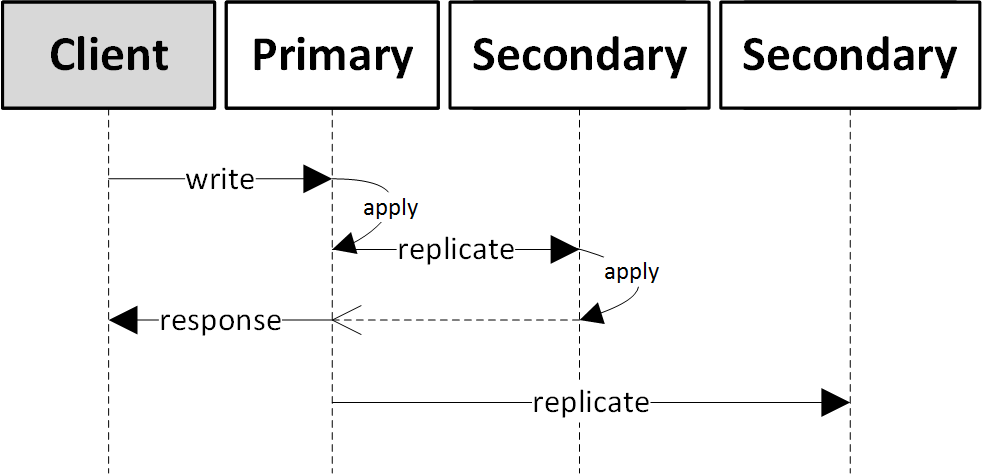
\includegraphics[width=\linewidth,keepaspectratio]{images/write-concern.png}
\caption{Write process with write concerns}
\label{write-concerns}
\end{figure}
\textit{Read preferences} allow the administrator to route read operations. They determine from which node a client is allowed to read. MongoDB supports five read preferences:
\begin{itemize}
  \item \textbf{primary:} all read operations are requested to the primary node
  \item \textbf{primaryPreferred:} read operations are requested to secondaries, if the primary is unavailable
  \item \textbf{secondary:} read operations are requested to secondaries
  \item \textbf{secondaryPreferred:} read operation are just requested to primary, if no secondary is available
  \item \textbf{nearest:} read operations are requested to the node with the lowest network latency
\end{itemize}
\cite{mdbdocu}
\subsection{Sharding}\label{mdb-sharding}
If the amount of data exceeds the capacity of a single database server, partitioning is needed to distribute the data on multiple servers. For MongoDB this ability is even more important, because it uses memory mapped file I/O to access its underlining data storage \cite{Hows2013}. MongoDB uses a horizontal partitioning mechanism called \textit{sharding}.\\
The data collection gets divided and distributed onto multiple servers called shards. Every shard is an independent database managed by multiple \textit{mongod} processes. All the shards are combined to one logical database. The partitioning and routing are managed by the earlier mentioned \textit{mongos} (\ref{mdb-core}) process. All write and read requests of an application are send to a \textit{mongos} process, that holds the information where the requested data is stored and forwards the requests to the responsible \textit{mongod} processes. The data is distributed based on a configured \textit{shard key} and chunk size. The metadata of a sharded cluster is stored on special config servers, where the \textit{mongos} processes can obtain the routing information \cite{Edward2015,Hows2013}.

\subsection{Summary}
Figure \ref{arch-example} describes one possible deployment architecture, that contains all in this section mentioned artifacts. Clients can connect to a \textit{mongos} process, running on an application server. This process forwards the requests, based on the information stored on the \textit{config servers}, to the right shard. A shard is an replica set, containing several \textit{mongod} processes. The \textit{shard key} in this example is the year. So Shard-1 contains all data from 1999 til 2009 and Shard-2 contains the data from 2009 til now. 
\begin{figure}[H]
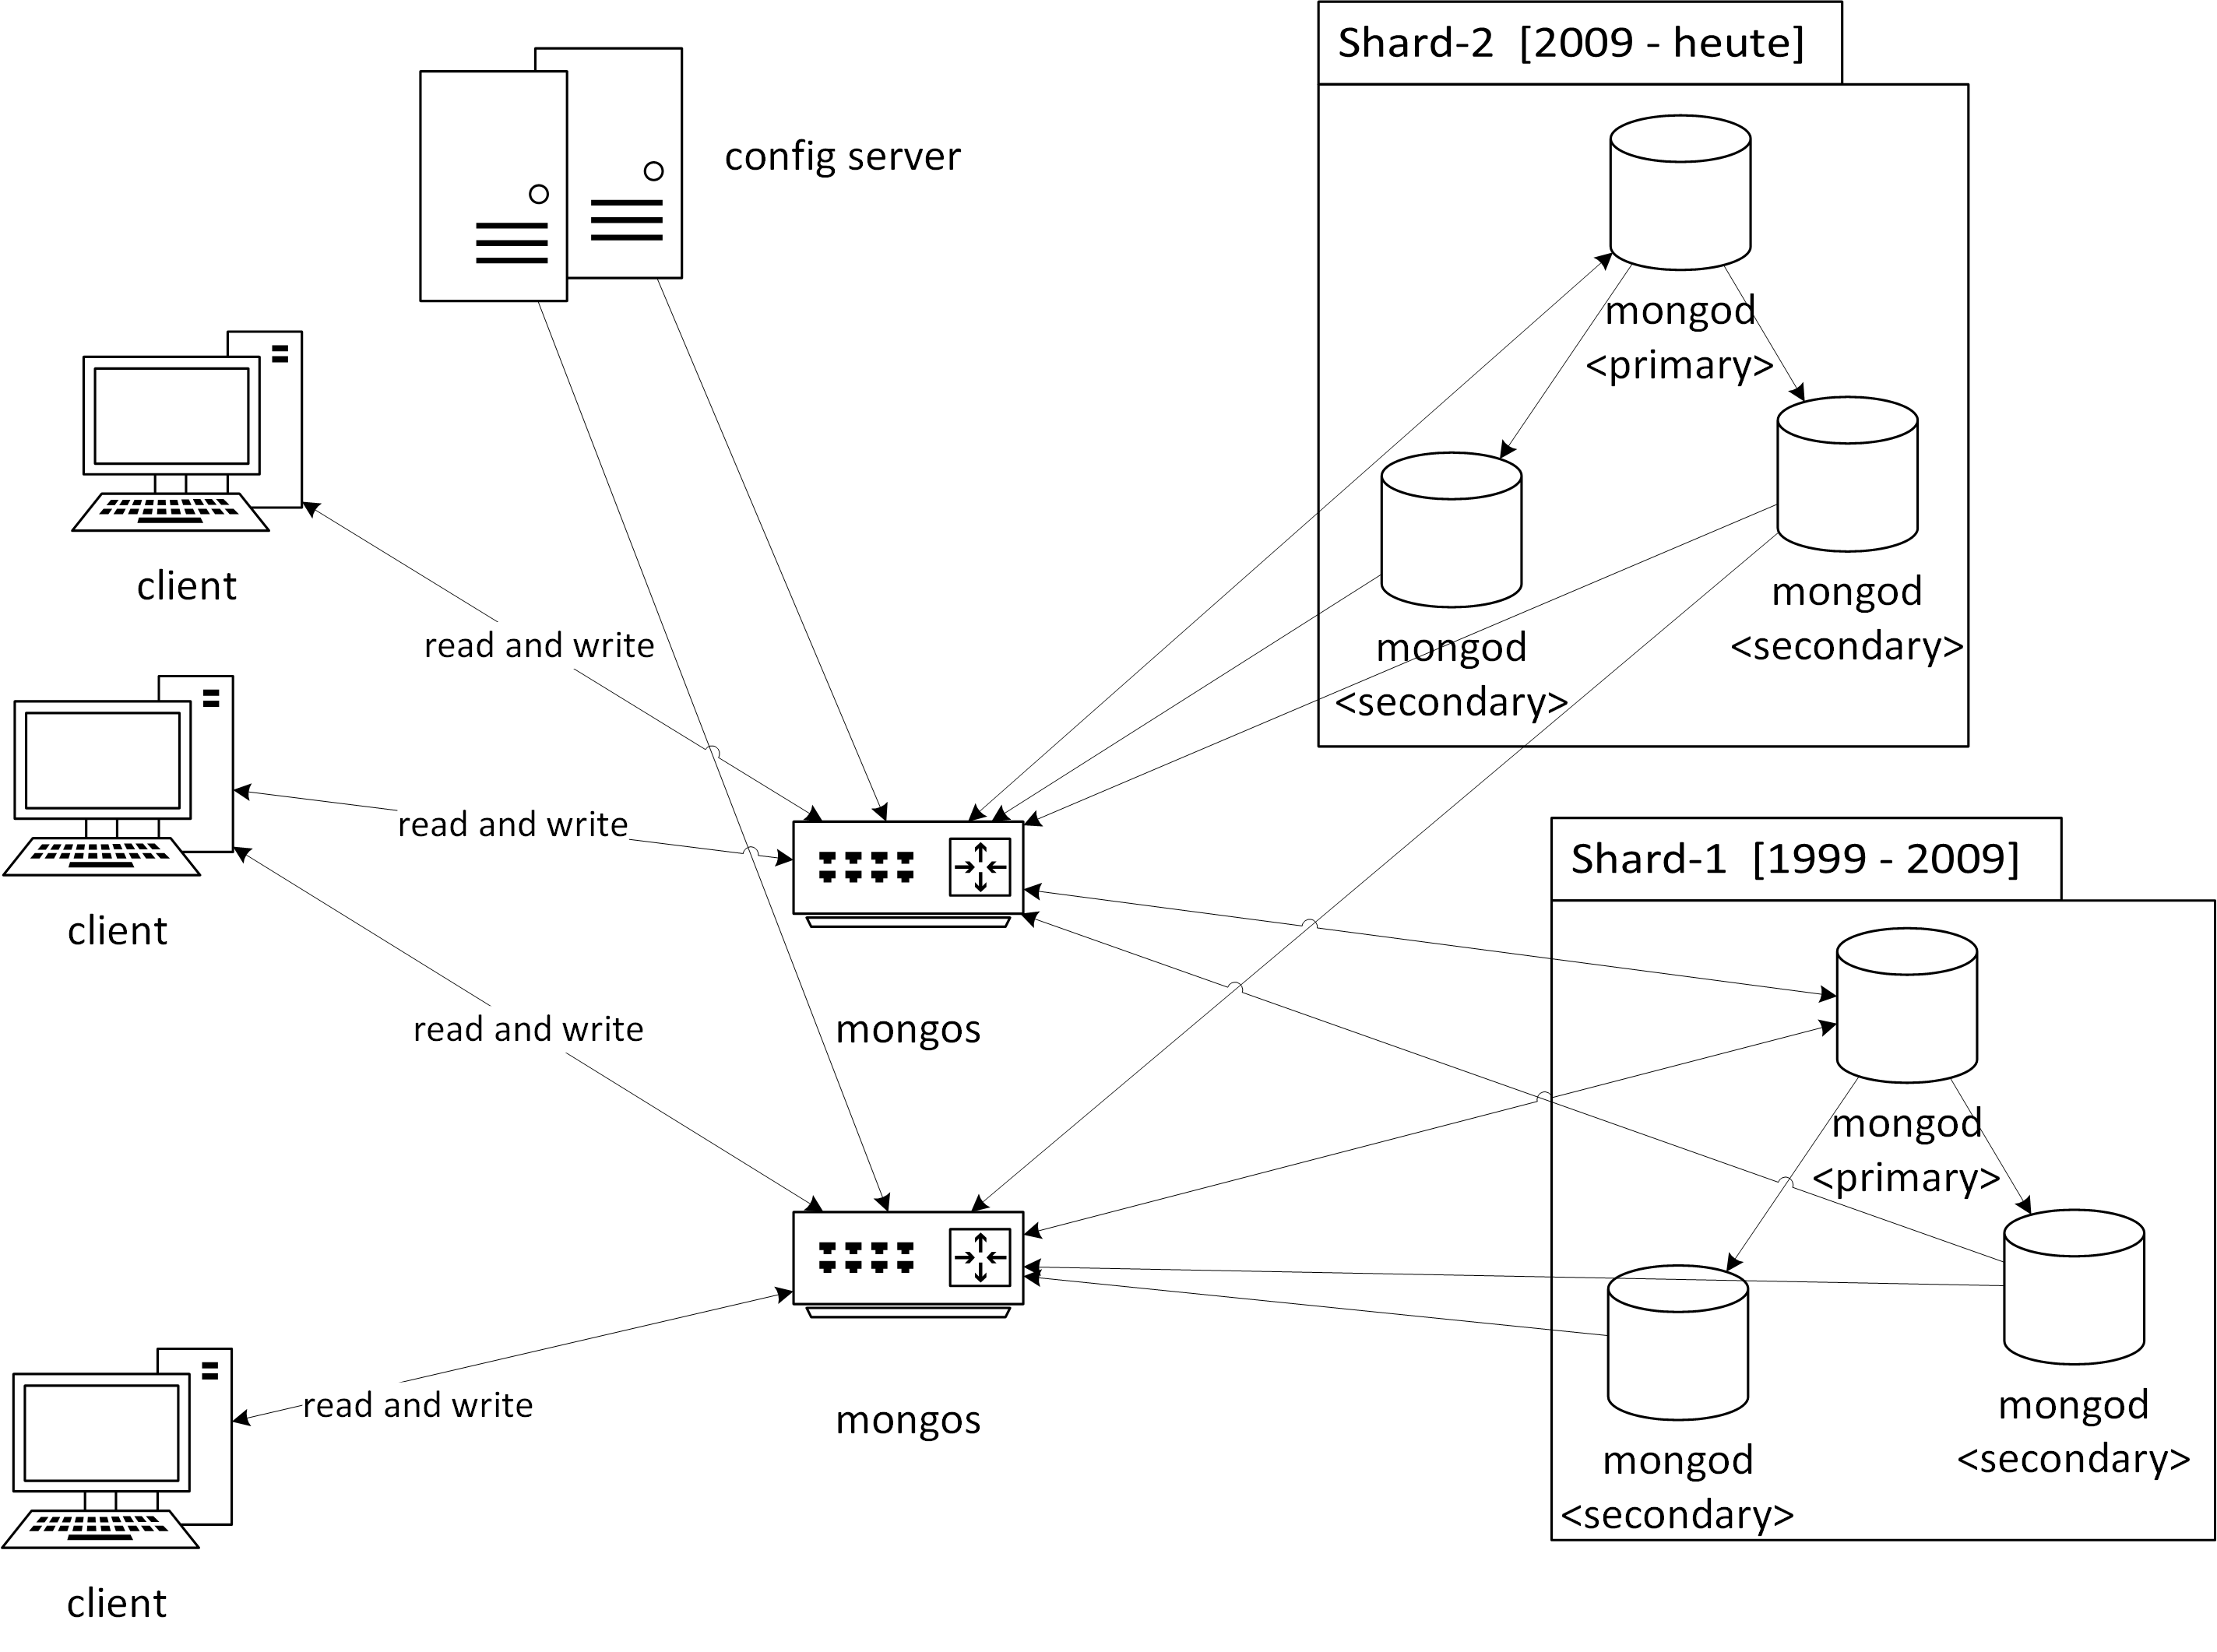
\includegraphics[width=\linewidth,keepaspectratio]{images/sharding.png}
\caption{MongoDB Architecture Example}
\label{arch-example}
\end{figure}
